\documentclass[10pt]{beamer}
\usetheme{Singapore}
\usepackage[utf8]{inputenc}
\usepackage{amsmath}
\usepackage{amsfonts}
\usepackage{amssymb}
%\author{}
%\title{}
%\setbeamercovered{transparent} 
%\setbeamertemplate{navigation symbols}{} 
%\logo{} 
%\institute{} 
%\date{} 
%\subject{} 
\title{Ideas to Death Star}
%\subtitle{Jr. Data Engineer}
\author{F.E. Charry-Pastrana, Jr. Data Engineer, Ventagium}
%\institute{Overleaf}
\date{2021.08.02}

\usepackage{ragged2e}

\apptocmd{\frame}{}{\justifying}{} % Allow optional arguments after frame.

\begin{document}

\begin{frame}
\titlepage
\end{frame}

%\begin{frame}
%\tableofcontents
%\end{frame}

\begin{frame}{}
\begin{center}
From
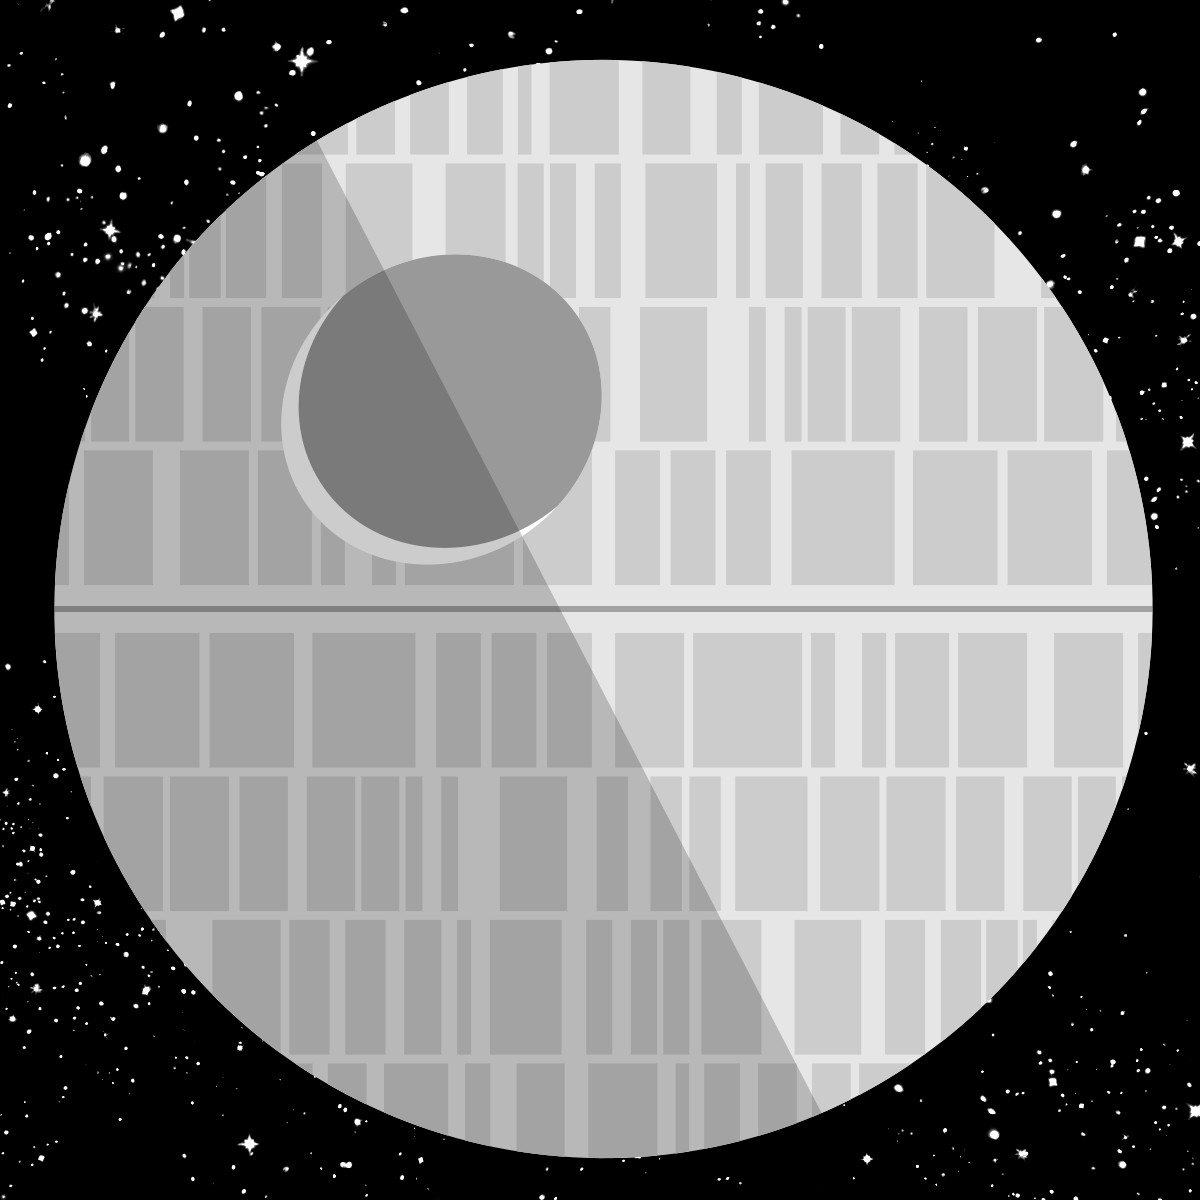
\includegraphics[width=40mm,scale=1.5]{img_2/death-star.png}
to
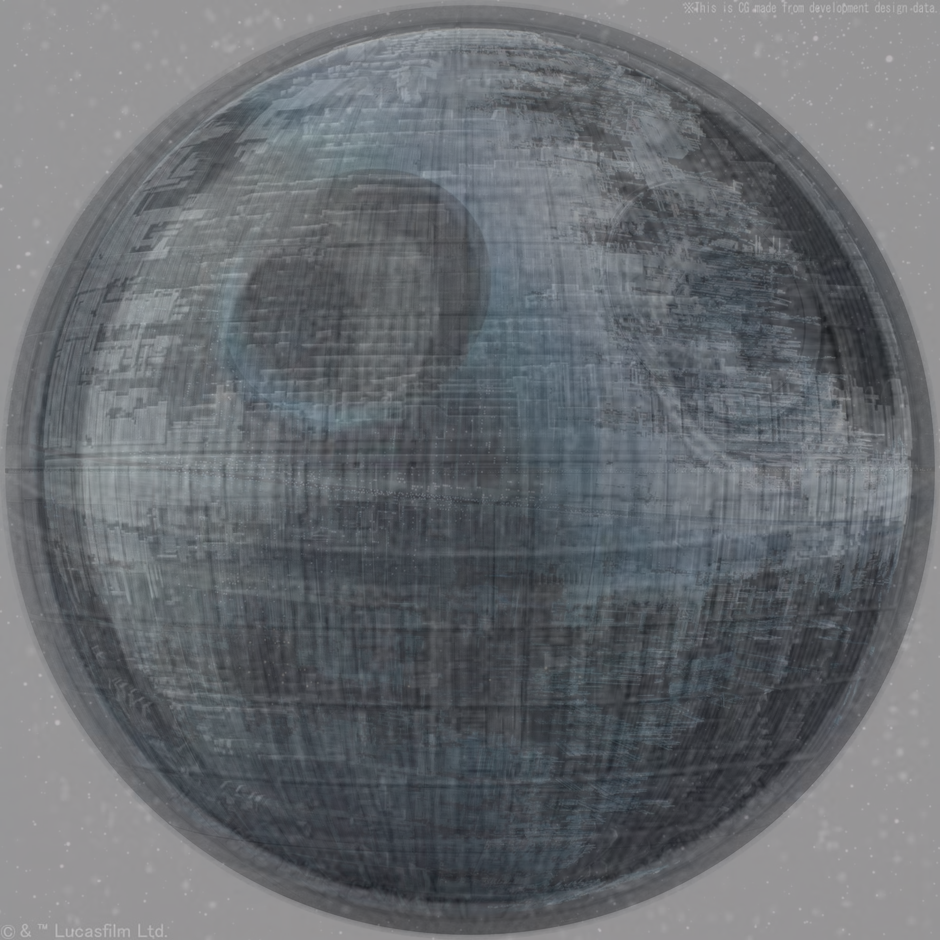
\includegraphics[width=40mm,scale=1.5]{img_2/death_1.png}? 
\end{center}
\end{frame}

\begin{frame}{}
\begin{center}
From
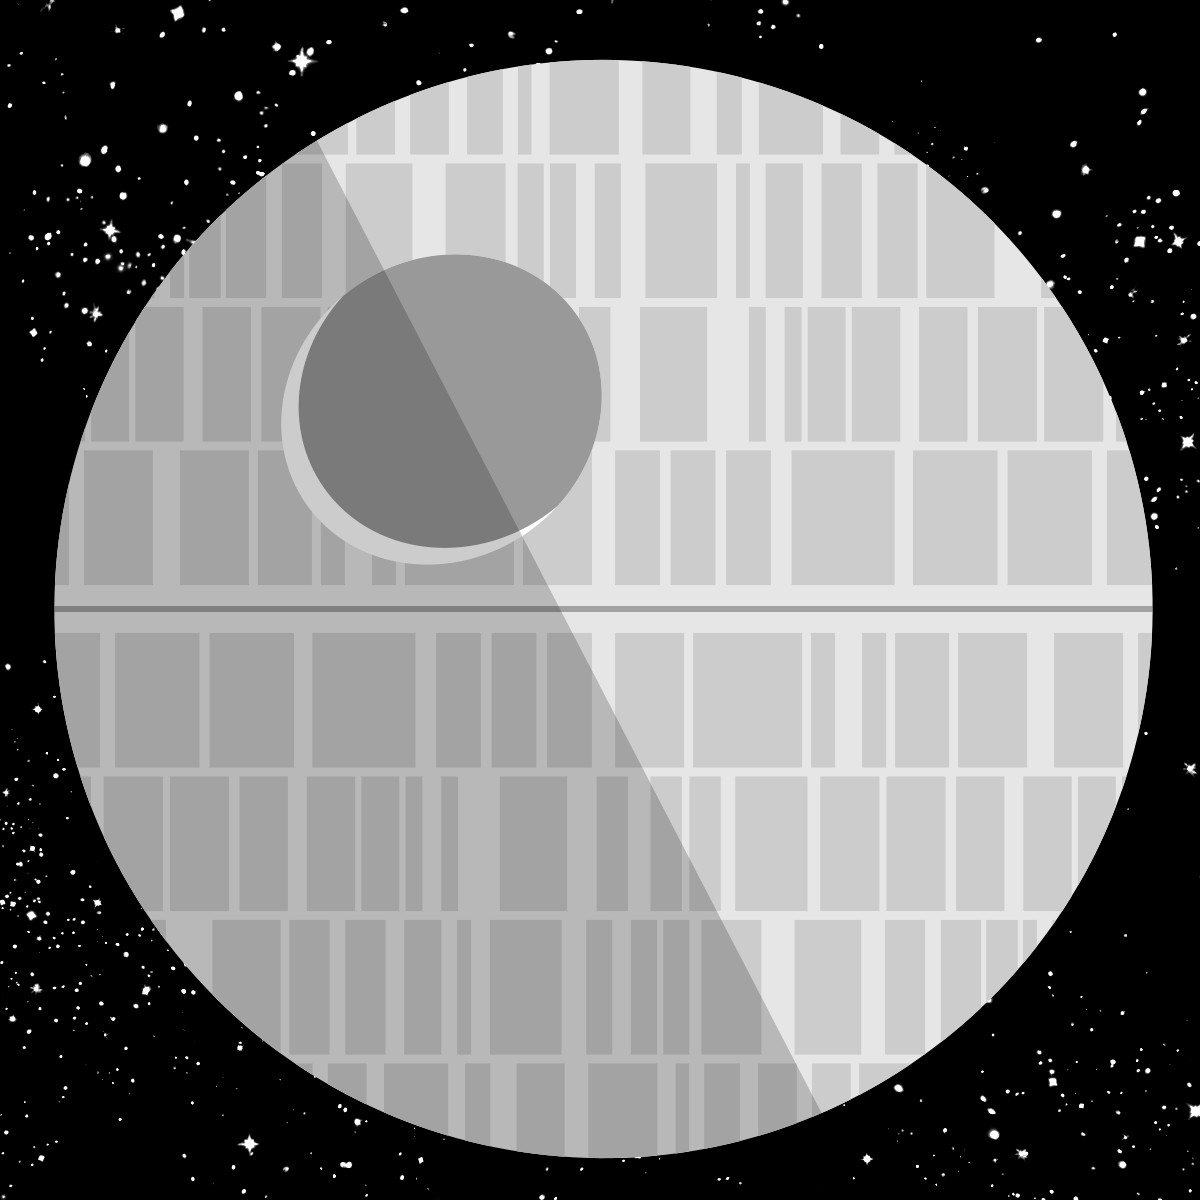
\includegraphics[width=30mm,scale=1.5]{img_2/death-star.png}
to\vspace{0.5cm}\\
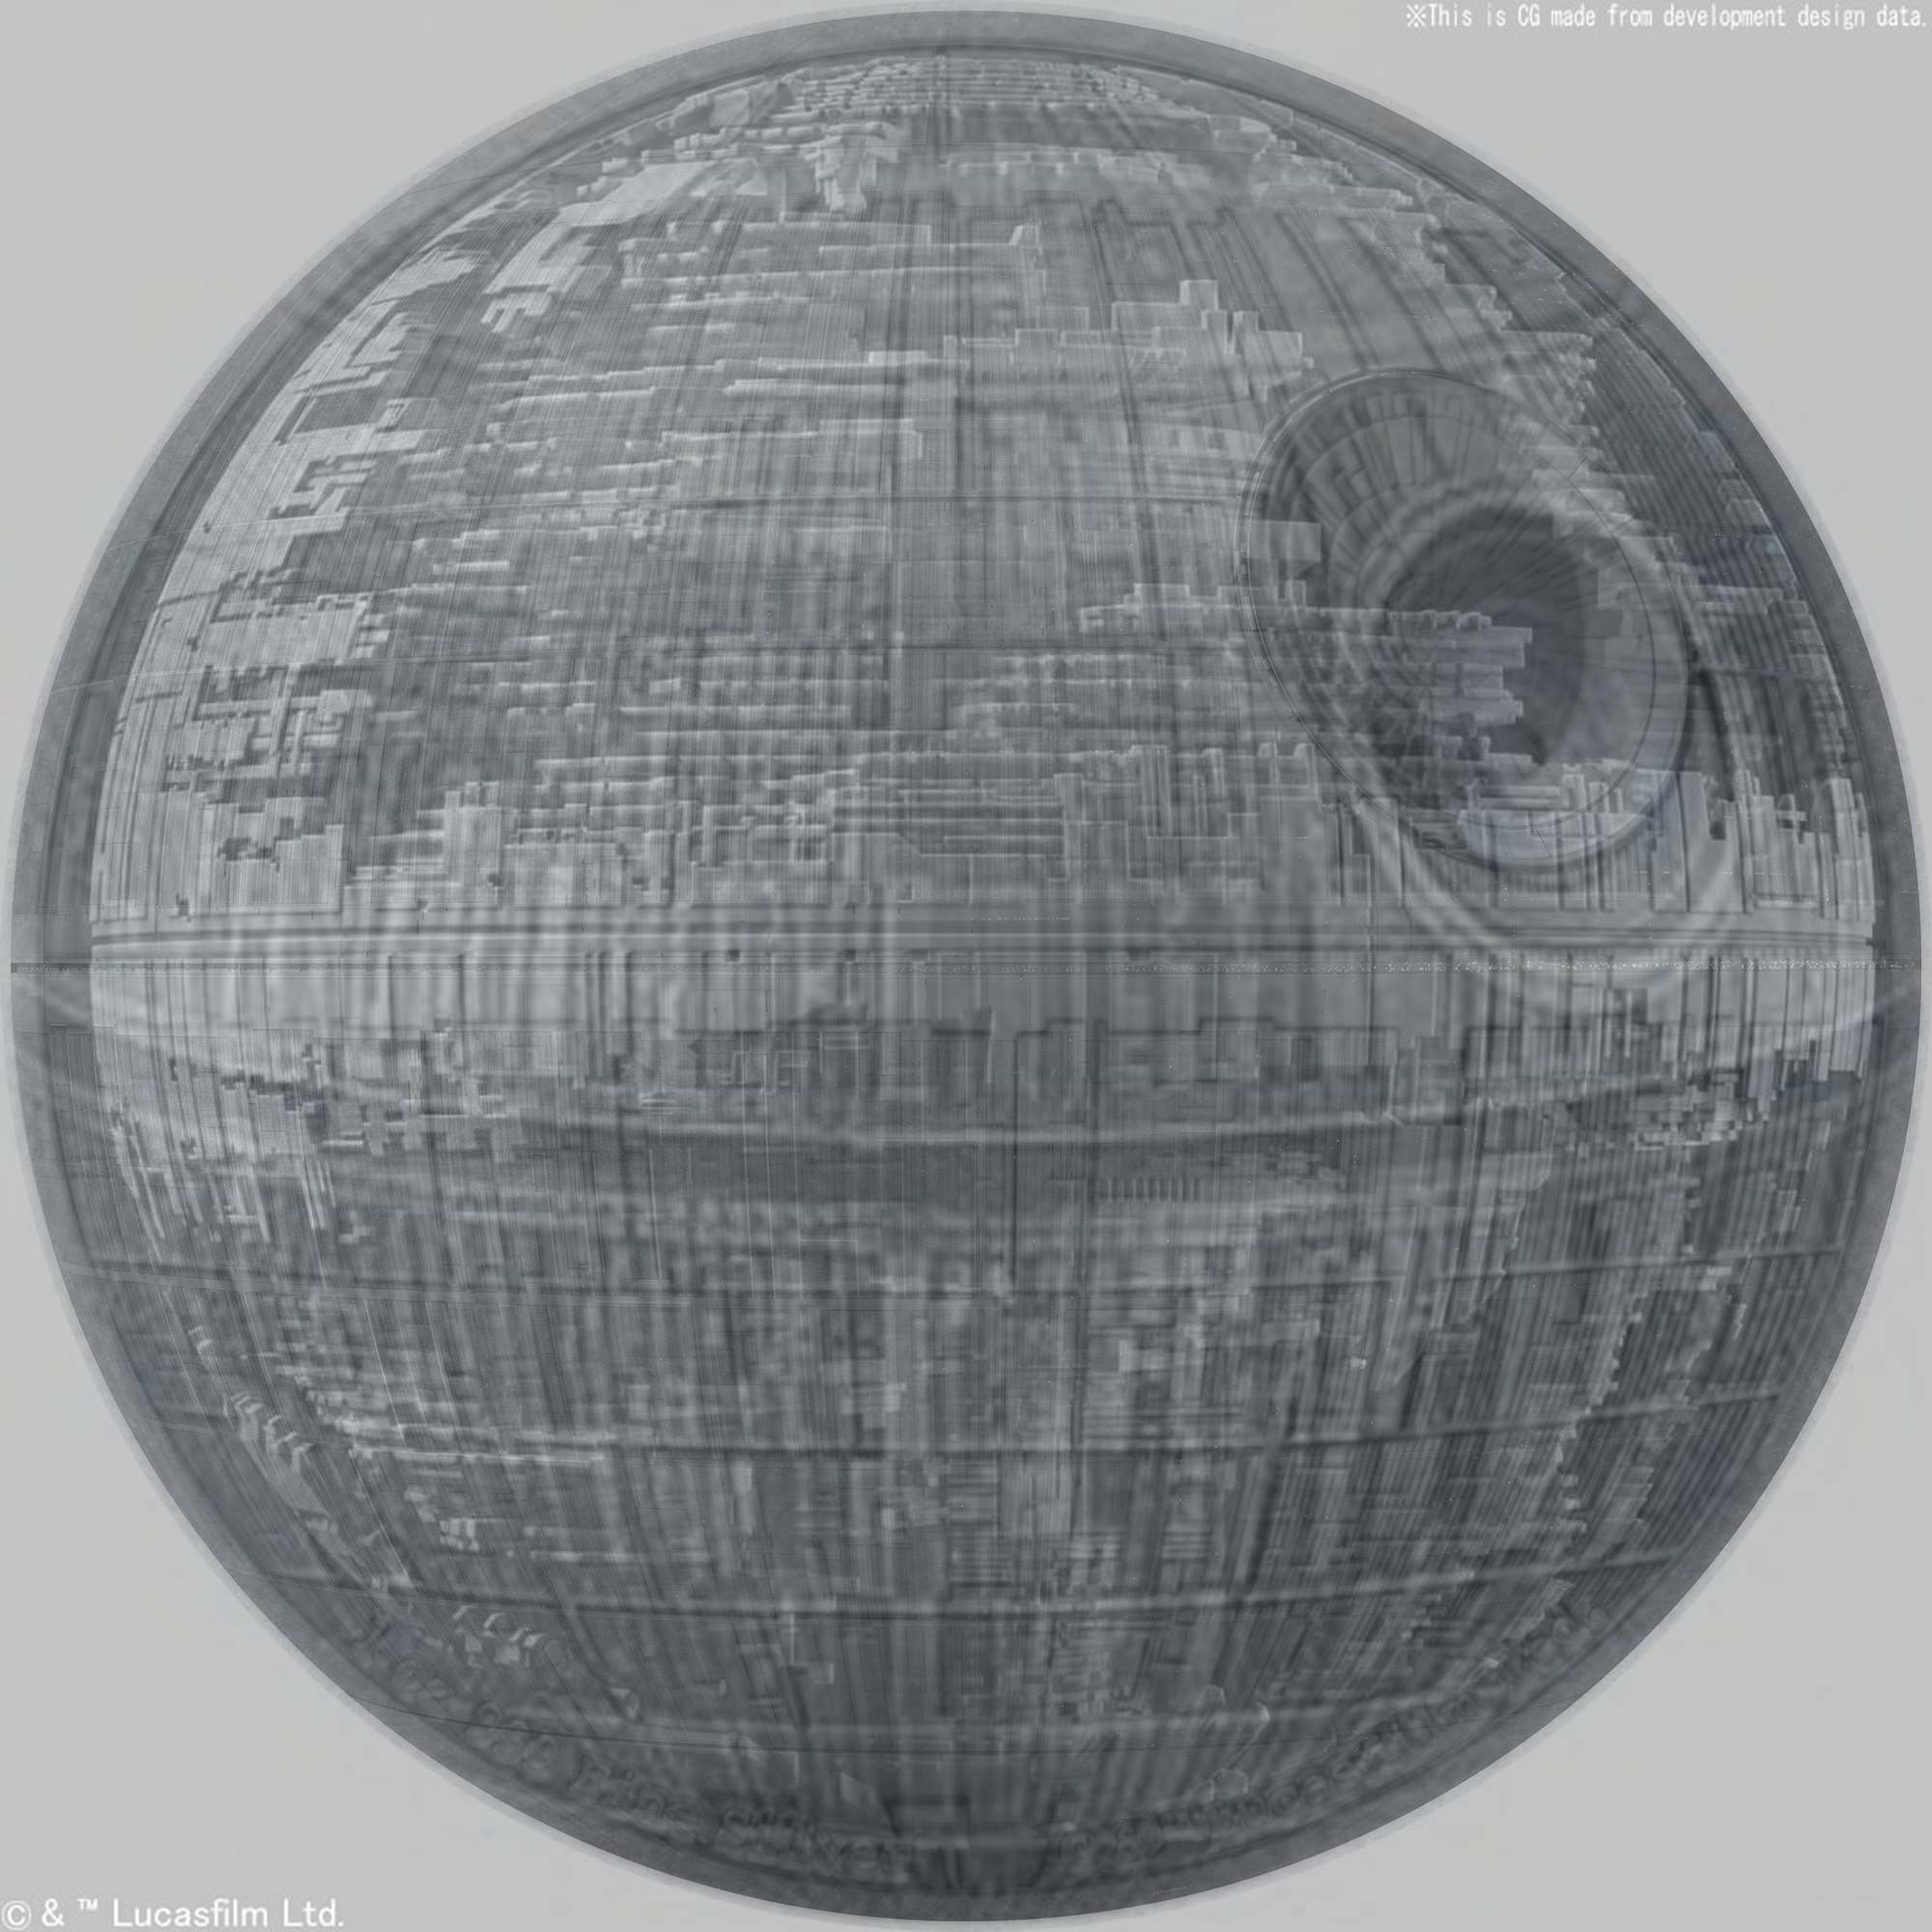
\includegraphics[width=40mm,scale=1.5]{img_2/death_1_1.png}
and
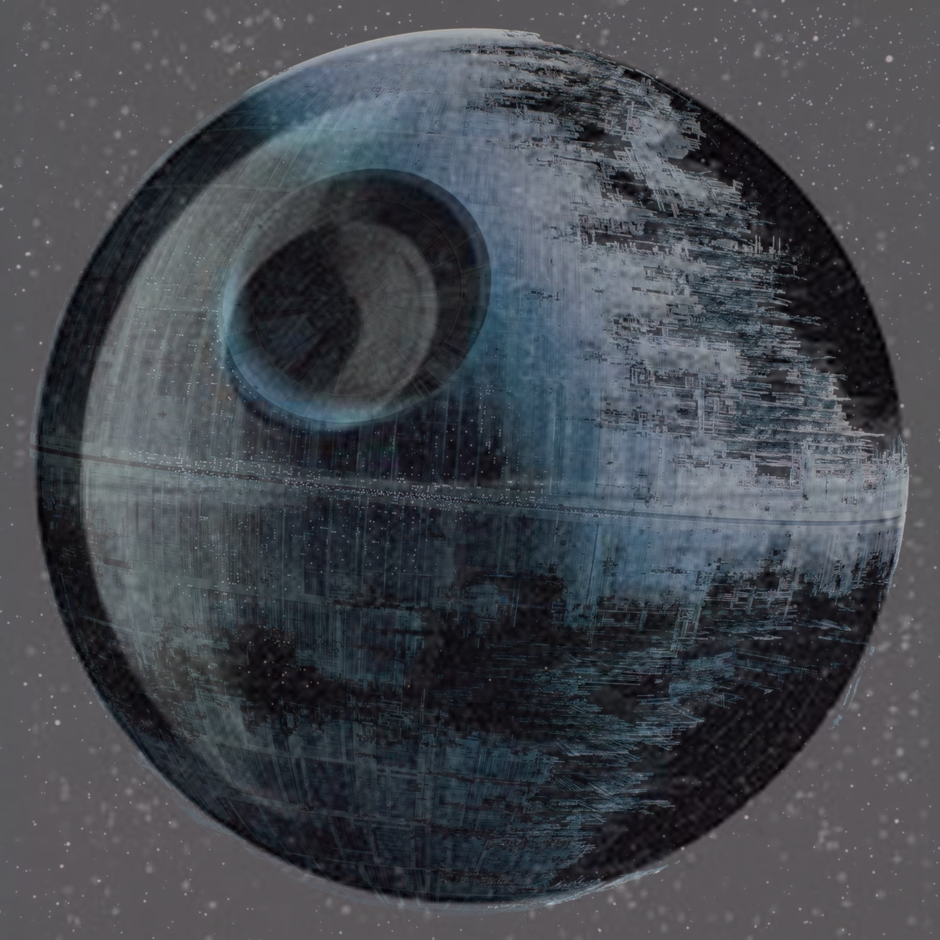
\includegraphics[width=40mm,scale=1.5]{img_2/death_1_2.png}.
\end{center}
\end{frame}

\begin{frame}{\textbf{No patterns,} \textbf{no symmetries}, just reality: just the future!}
\begin{center}
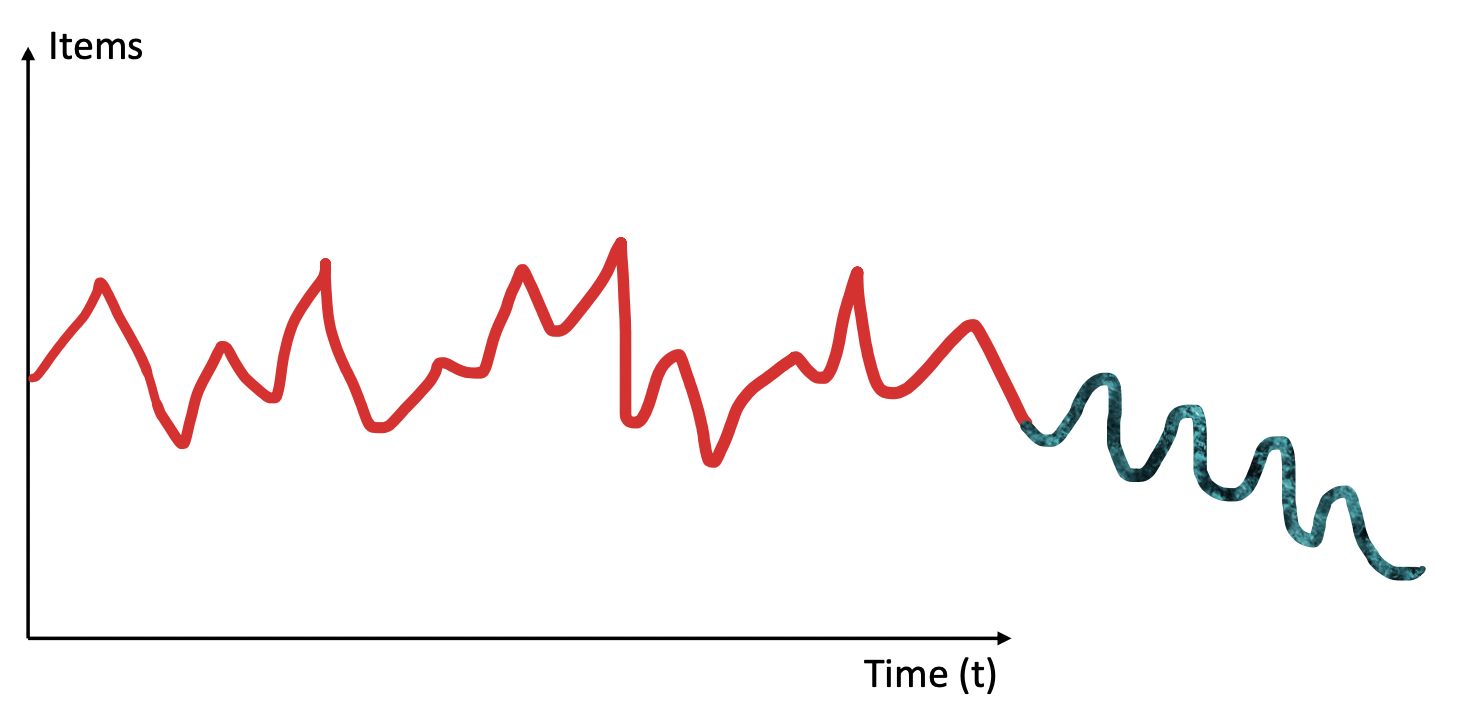
\includegraphics[height=20mm,scale=1.5]{img_2/1.png}
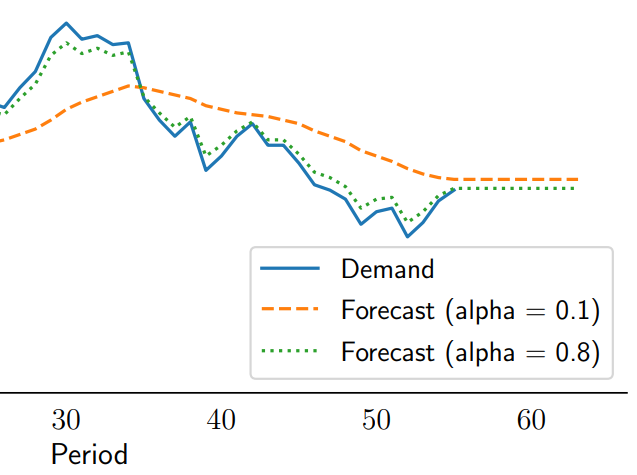
\includegraphics[height=20mm,scale=1.5]{img_2/2.png}
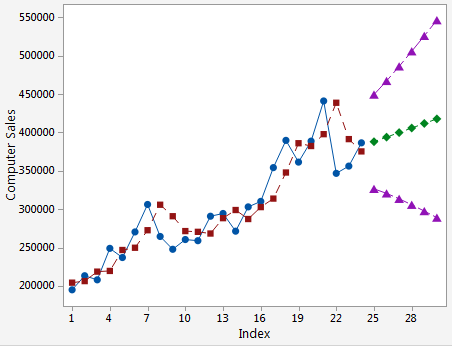
\includegraphics[height=20mm,scale=1.5]{img_2/3.png}
Exponential smoothing + error
\end{center}
\end{frame}

\begin{frame}{Velocity = items = items$\times$profit?}
\begin{columns}
\begin{column}{0.38\textwidth}  %%<--- here
    \begin{figure}
    \centering
     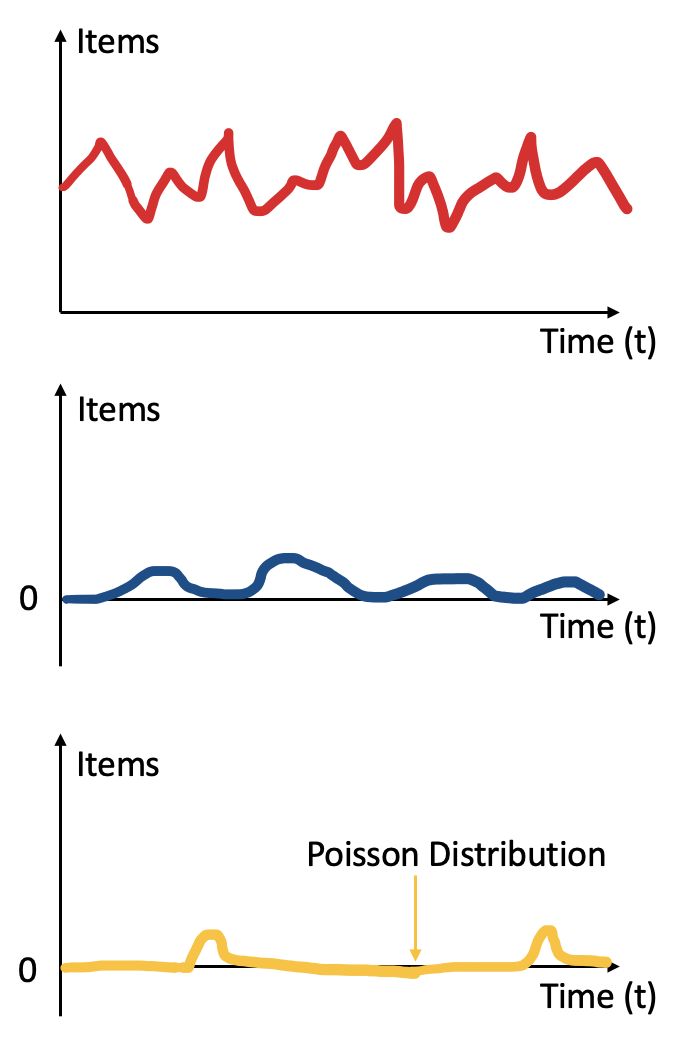
\includegraphics[scale=0.3]{img_2/4.png}
     \end{figure}
\begin{center}
ABC
\end{center}
\end{column}
\begin{column}{0.65\textwidth}
\begin{figure}
\centering
     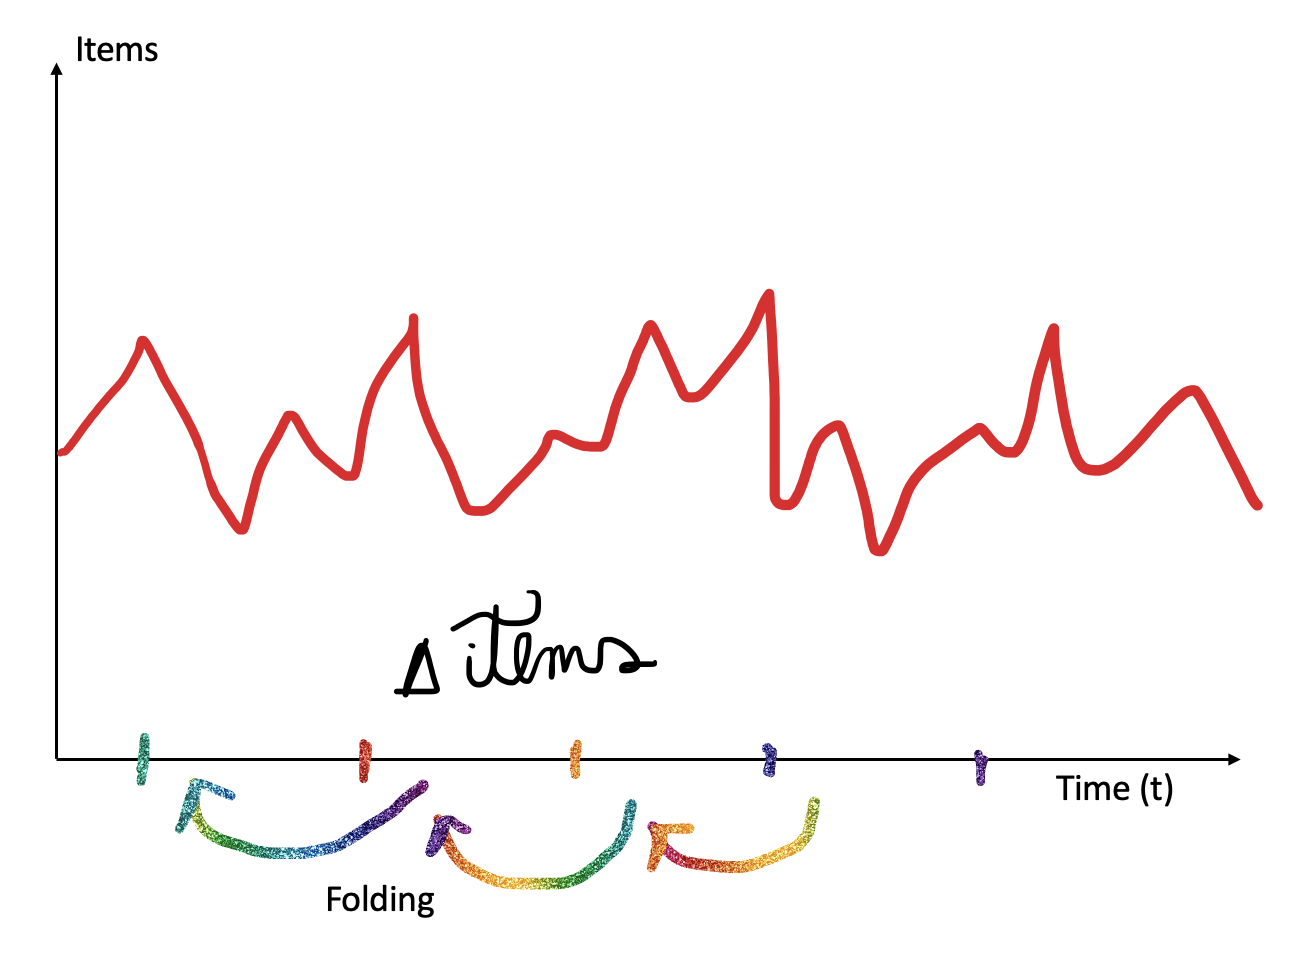
\includegraphics[height=30mm]{img_2/5.png}
\end{figure}
\begin{center}
Error prediction?
\end{center}
\begin{figure}
\centering
     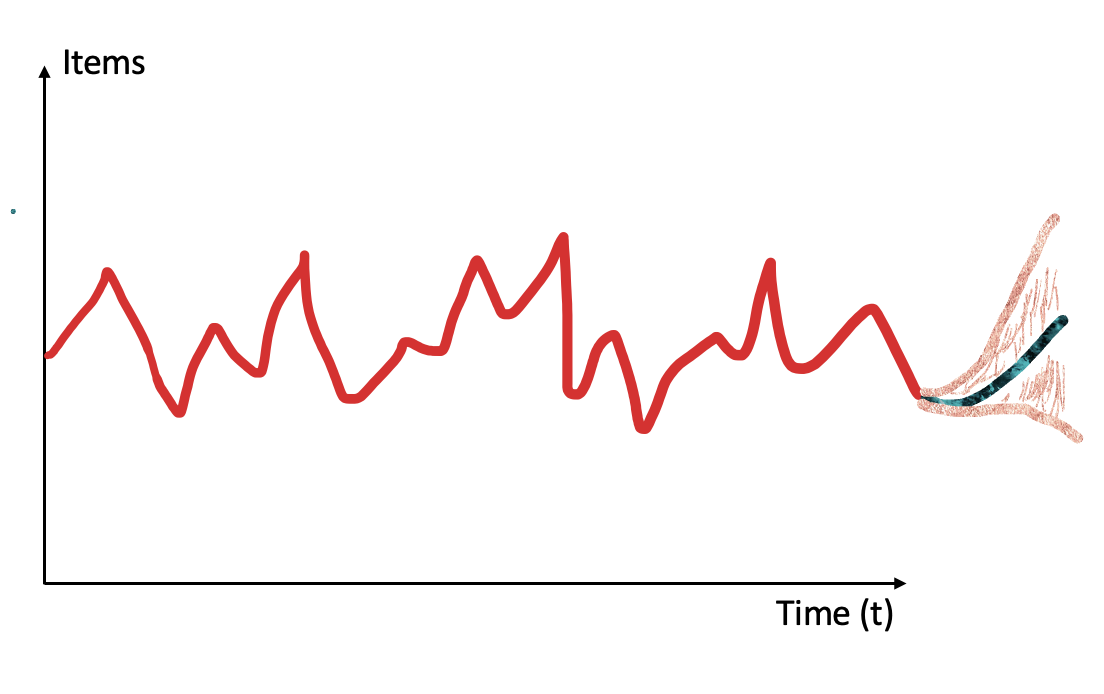
\includegraphics[height=30mm]{img_2/6.png}
\end{figure}
\end{column}
\end{columns}
\end{frame}

\end{document}